\chapter{Problem Setup}
\label{ch2}

\section{Physical Experimental Setup}
\subsection{Spatial Proximity}
Show Google Maps screenshot of MZA office (location of weather station), Fitz Hall (location of DELTA), and Y-Tower (location of target). Overlay arrow from Fitz Hall pointing to the Y-Tower. Overlay text boxes with relevant location (LLA) information.

\begin{figure}[h!]
	\centering
	\includegraphics[width=0.99\textwidth]
	{DELTA_Path.png}
	\hfill
	\caption{Fitz Hall to Y-Tower geometry. \textbf{NEED TO EXPAND MAP TO INCLUDE WEATHER STATION}}
	\label{fig:test3}
\end{figure}

\begin{figure}[h!]
	\centering
	\subfloat[Telescope setup\label{fig:test_a}]{
		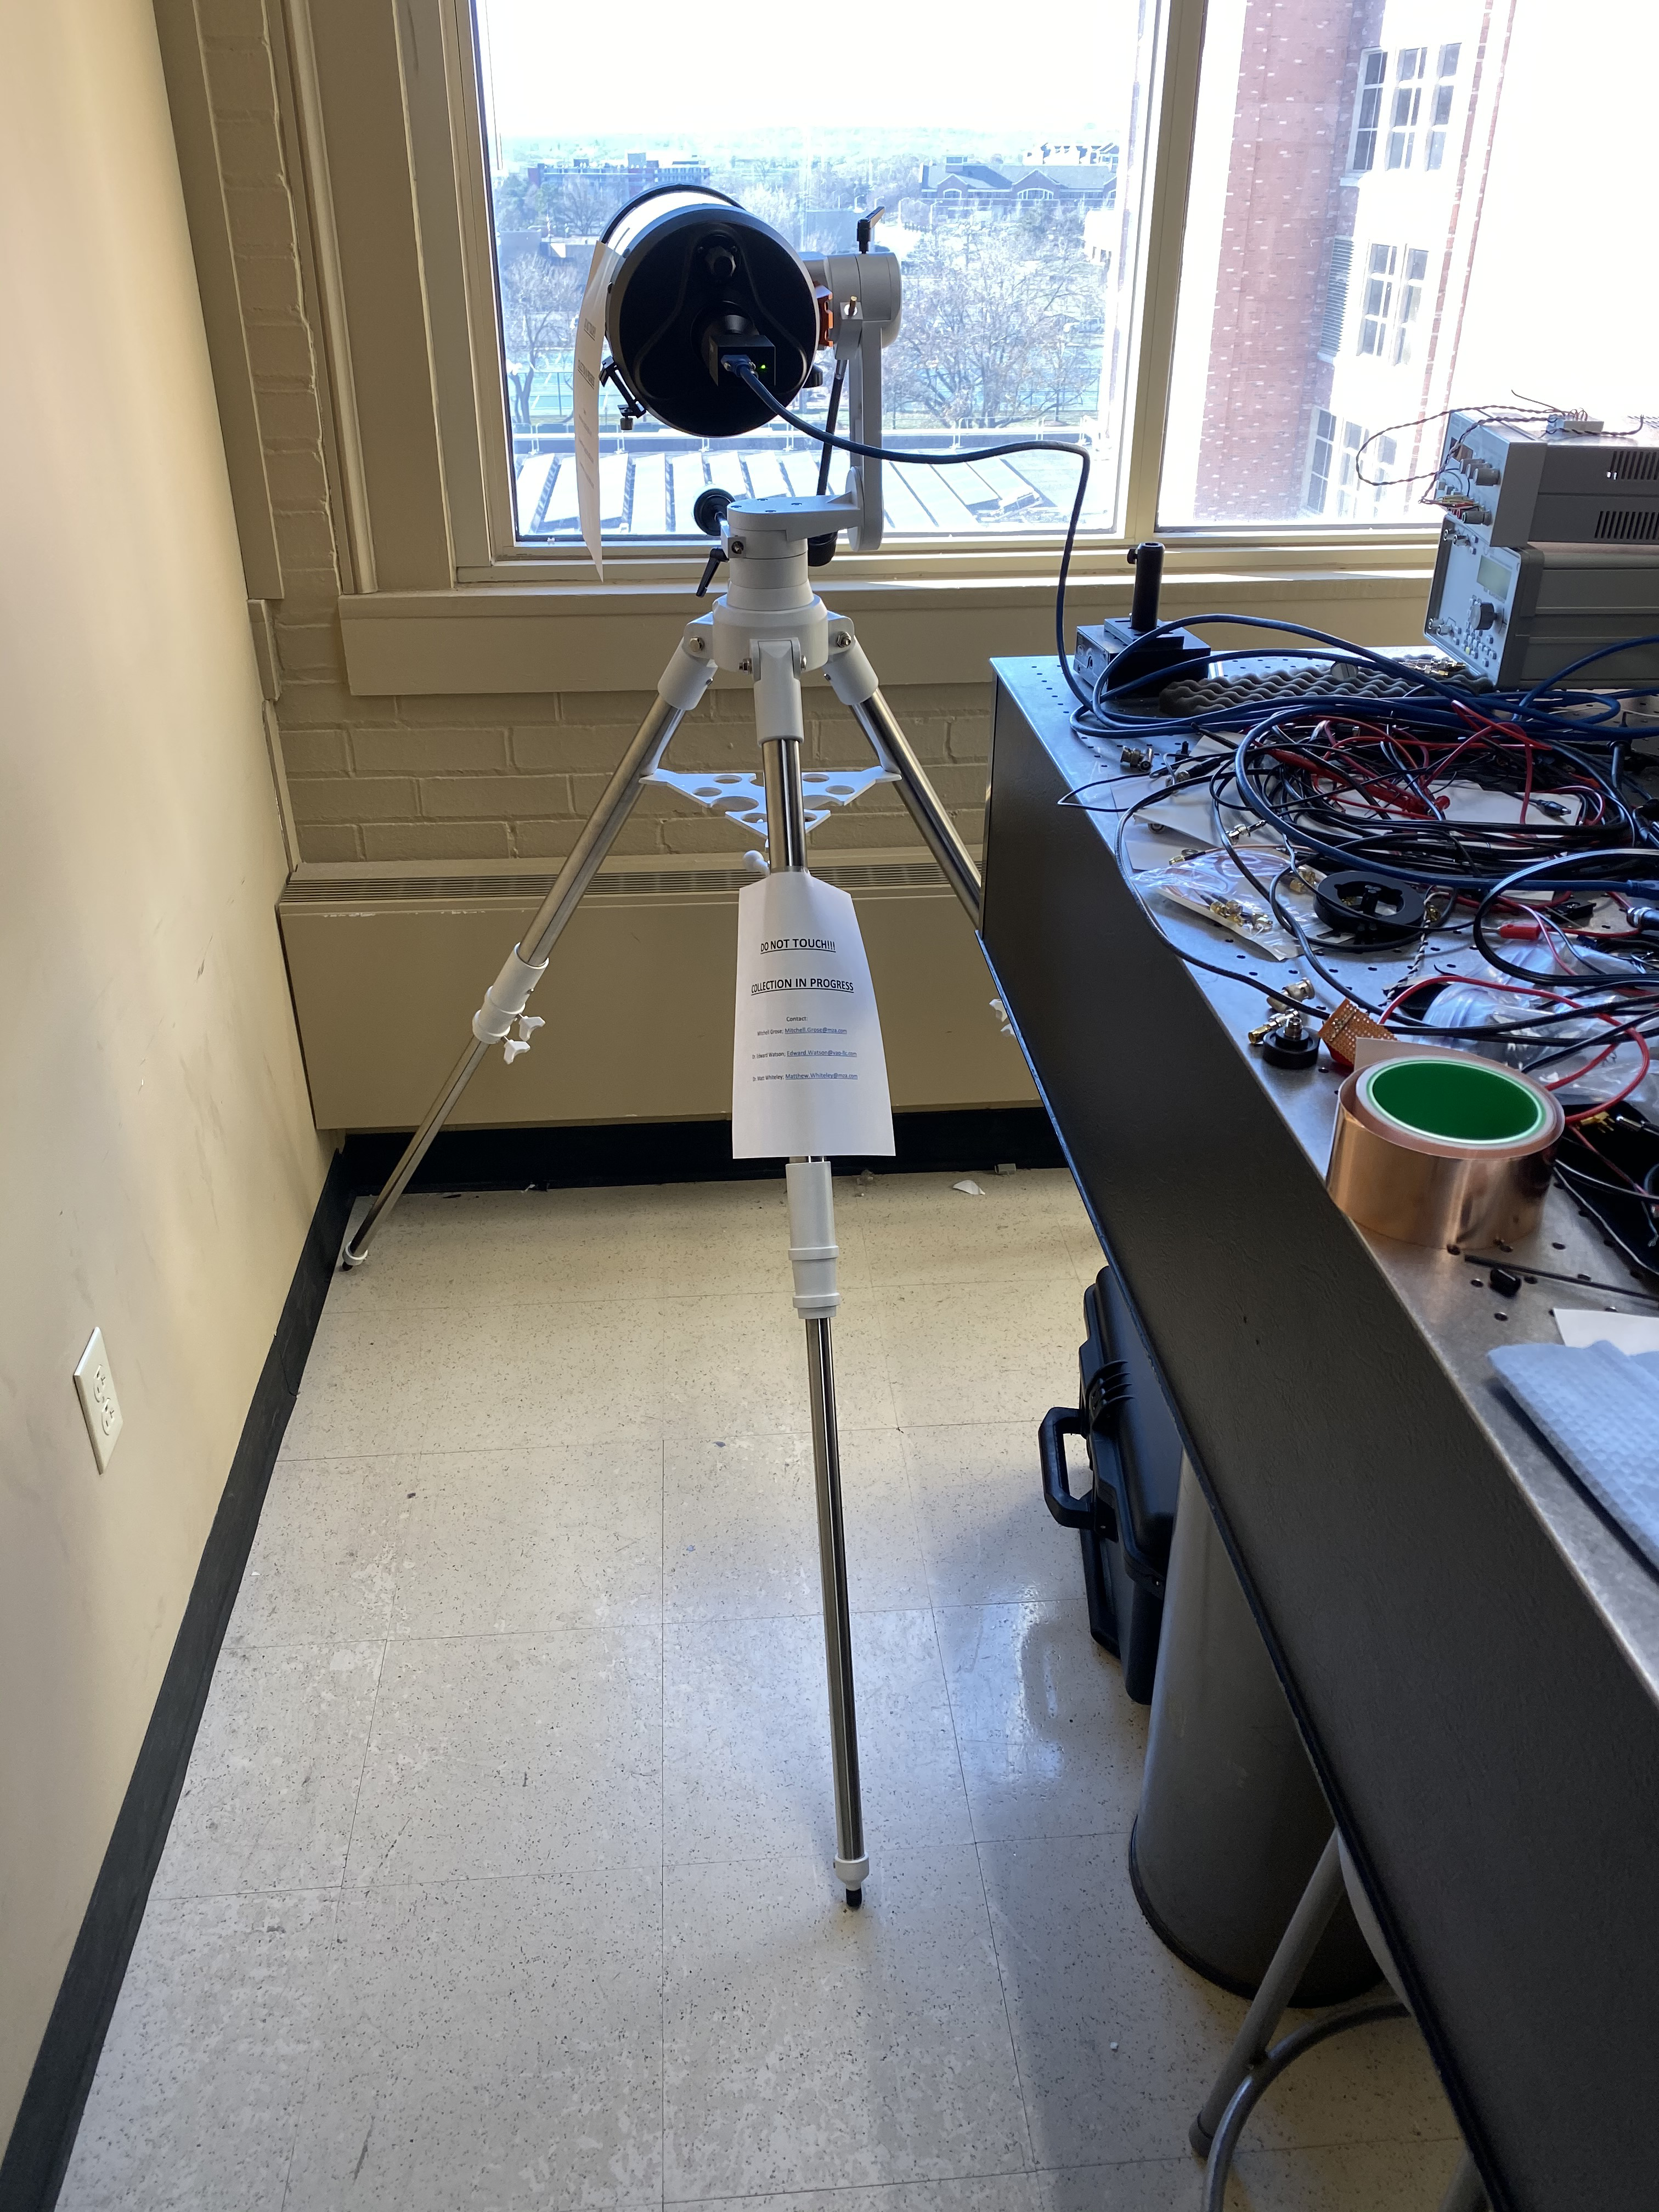
\includegraphics[width=0.49\textwidth, angle=-90]
		{DELTA_setup1.jpg}
	}
	\subfloat[Wide view of target\label{fig:test_b}]{
		\includegraphics[width=0.49\textwidth, angle=-90]
		{DELTA_setup3.jpg}
	}
	\hfill
	\subfloat[View of target through the DELTA telescope\label{fig:test_c}]{
		\includegraphics[width=0.49\textwidth]
		{Y_Tower.jpg}
	}
	\hfill
	\caption{DELTA setup for collection of minute-by-minute $C_{n}^{2}$ measurements.}
	\label{fig:test}
\end{figure}

\section{Modeling Experimental Setup}
Finding best model to forecast 4 hours of turbulence conditions from prior environmental measurements.
\subsection{Data Processing (Ch. 3)}
\subsection{Grid Search (Ch. 4)}
Architectures, sequence length, number of layers, number of nodes per layer.
\subsubsection{Statistical Analysis of Grid Search}
\subsection{Application of ``Best" Model to Test Dataset (Ch. 5)}